 \documentclass{article}

\usepackage{fancyhdr}
\usepackage{extramarks}
\usepackage{amsmath}
\usepackage{amsthm}
\usepackage{amsfonts}
\usepackage{amssymb}
\usepackage{xparse}
\usepackage{tikz}
\usepackage{graphicx}
\usepackage[plain]{algorithm}
\usepackage{algpseudocode}
\usepackage{listings}
\usepackage{hyperref}
\usepackage[per-mode = fraction]{siunitx}
\usepackage{calc}

\usetikzlibrary{automata,positioning}

\hypersetup{
    colorlinks=true,
    linkcolor=blue,
    filecolor=magenta,
    urlcolor=blue,
    }

\urlstyle{same}

%
% Basic Document Settings
%

\topmargin=-0.45in
\evensidemargin=0in
\oddsidemargin=0in
\textwidth=6.5in
\textheight=9.0in
\headsep=0.25in

\linespread{1.1}

\pagestyle{fancy}
\lhead{\hmwkAuthorName}
\chead{\hmwkClass\ (\hmwkClassInstructor,\ \hmwkClassTime): \hmwkTitle}
\rhead{\firstxmark}
\lfoot{\lastxmark}
\cfoot{\thepage}

\renewcommand\headrulewidth{0.4pt}
\renewcommand\footrulewidth{0.4pt}

\setlength\parindent{0pt}
\allowdisplaybreaks
%
% Title Page
%

\title{
	\vspace{2in}
	\textmd{\textbf{\hmwkClass:\ \hmwkTitle}}\\
	\normalsize\vspace{0.1in}\small{Due\ on\ \hmwkDueDate\ at \hmwkDueTime}\\
	\vspace{0.1in}\large{\textit{\hmwkClassInstructor,\ \hmwkClassTime}}
	\vspace{3in}
}
\author{\textbf{\hmwkAuthorName}}
\date{\hmwkCompletionDate}

%
% Create Problem Sections
%

\newcommand{\enterProblemHeader}[1]{
	\nobreak\extramarks{}{Problem #1 continued on next page\ldots}\nobreak{}
	\nobreak\extramarks{Problem #1 (continued)}{Problem #1 continued on next page\ldots}\nobreak{}
}

\newcommand{\exitProblemHeader}[1]{
	\nobreak\extramarks{Problem #1 (continued)}{Problem #1 continued on next page\ldots}\nobreak{}
	\nobreak\extramarks{Problem #1}{}\nobreak{}
}

%
% Homework Problem Environment
%
\NewDocumentEnvironment{hwkProblem}{m m s}{
	\section*{Problem #1: #2}
	\enterProblemHeader{#1}
	\setcounter{partCounter}{1}
}{
	\exitProblemHeader{#1}
	\IfBooleanF{#3} % if star, no new page
		{\newpage}
}

% Alias for the Solution section header
\newcommand{\hwkSol}{\vspace{\baselineskip / 2}\textbf{\Large Solution}\vspace{\baselineskip / 2}}

% Alias for the Solution Part subsection header
\newcounter{partCounter}
\newcommand{\hwkPart}{
	\vspace{\baselineskip / 2}
	\textbf{\large Part \Alph{partCounter}}
	\vspace{\baselineskip / 2}
	\stepcounter{partCounter}
}

%
% Various Helper Commands
%

% Such That
\newcommand{\st}{\text{s.t.}}

% Useful for algorithms
\newcommand{\alg}[1]{\textsc{\bfseries \footnotesize #1}}

% For derivatives
\newcommand{\deriv}[1]{\frac{\mathrm{d}}{\mathrm{d}x} (#1)}

% For partial derivatives
\newcommand{\pderiv}[2]{\frac{\partial}{\partial #1} (#2)}

% Integral dx
\newcommand{\dx}{\mathrm{d}x}
\newcommand{\dy}{\mathrm{d}y}

% Probability commands: Expectation, Variance, Covariance, Bias
\newcommand{\e}[1]{\mathrm{e}#1}
\newcommand{\E}{\mathrm{E}}
\newcommand{\Var}{\mathrm{Var}}
\newcommand{\Cov}{\mathrm{Cov}}
\newcommand{\Bias}{\mathrm{Bias}}

% Defining Units that are not in the SI base
\DeclareSIUnit\bar{bar}
\DeclareSIUnit\ft{ft}
\DeclareSIUnit\dollar{\$}
\DeclareSIUnit\cent{\text{\textcent}}
\DeclareSIUnit\c{\degreeCelsius}

% Code Listing config
\usepackage{xcolor}
\definecolor{codegreen}{rgb}{0,0.6,0}
\definecolor{codegray}{rgb}{0.5,0.5,0.5}
\definecolor{codepurple}{rgb}{0.58,0,0.82}
\definecolor{backcolour}{rgb}{0.95,0.95,0.92}
\lstdefinestyle{overleaf}{
	% backgroundcolor=\color{backcolour},
	commentstyle=\color{codegreen},
	keywordstyle=\color{magenta},
	numberstyle=\tiny\color{codegray},
	stringstyle=\color{codepurple},
	basicstyle=\ttfamily\footnotesize,
	breakatwhitespace=false,
	breaklines=true,
	captionpos=b,
	keepspaces=true,
	numbers=left,
	numbersep=5pt,
	showspaces=false,
	showstringspaces=false,
	showtabs=false,
	tabsize=4
}

\usepackage[latte]{catppuccinpalette}
\lstdefinestyle{catppuccin}{
	breaklines=true,
	keepspaces=true,
	numbers=left,
	numbersep=5pt,
	showspaces=false,
	showstringspaces=false,
	breakatwhitespace=true,
	tabsize=4,
	stringstyle = {\color{CtpGreen}},
	commentstyle={\color{CtpOverlay1}},
	basicstyle = {\small\color{CtpText}\ttfamily},
	keywordstyle = {\color{CtpMauve}},
	keywordstyle = [2]{\color{CtpBlue}},
	keywordstyle = [3]{\color{CtpYellow}},
	keywordstyle = [4]{\color{CtpLavender}},
	keywordstyle = [5]{\color{CtpPeach}},
	keywordstyle = [6]{\color{CtpTeal}}
}

\lstset{style=catppuccin}


%
% Homework Details
%   - Title
%   - Due date
%   - Due time
%   - Course
%   - Section/Time
%   - Instructor
%   - Author
%

\newcommand{\hmwkTitle}{Homework 01}
\newcommand{\hmwkDueDate}{September 10, 2024}
\newcommand{\hmwkDueTime}{05:00 PM}
\newcommand{\hmwkClass}{ENAE 311H}
\newcommand{\hmwkClassTime}{Section 0101}
\newcommand{\hmwkClassInstructor}{Dr. Brehm}
\newcommand{\hmwkAuthorName}{\textbf{Vai Srivastava}}
\newcommand{\hmwkCompletionDate}{September 10, 2024}

\begin{document}

\maketitle

\pagebreak

\begin{homeworkProblem}

	Consider an infinitely thin flat plate with a \( \qty{1}{\m} \) chord at an angle of attack of \ang{15} to an oncoming flow. The pressure distributions on the upper and lower surfaces are given by \( p_u = 2\e{4} \left( x - 1 \right) + 2.7\e4 \) and \( p_l = 1\e{4} \left( x - 1 \right) + 1.1\e{5} \), where \( x \) is the distance from the leading edge along the chord; the shear stress distributions are \( \tau_u = 144x^{-0.3} \) and \( \tau_l = 360 x^{-0.3} \). Here, the units of \( p \) and \( \tau \) are \unit{\N \per \square \m}. Calculate the normal and axial forces, the lift and drag, moments about the leading edge and quarter chord, all per unit span, as well as the center of pressure.

	\solution

	\part

	Normal Force is calculated here by integrating the pressure difference between the upper and lower faces over the chord length.
	\[
		N = \int_0^1 p_l(x)-p_u(x) \dx = \qty{88}{\kN}\qed
	\]

	\part

	Axial Force is calculated here by integrating the shear stress on the upper and lower faces over the chord length.
	\[
		A = \int_0^1 \tau_l(x)-\tau_u(x) \dx = \qty{720}{\N}\qed
	\]

	\part

	Lift is computed here using the Normal and Axial forces and the angle of attack \( \alpha \).
	\[
		L = N \cos{\alpha}-A\sin{\alpha} = \qty{81.81512}{\kN}\qed
	\]

	\part

	Drag is computed here using the Normal and Axial forces and the angle of attack \( \alpha \).
	\[
		D = A \cos{\alpha}+N\sin{\alpha} = \qty{23.47154}{\kN}\qed
	\]

	\part

	Moment about the leading edge is calculated here by integrating the pressure difference in the same way as we calculated the Normal Force, but also taking into account the position along the chord.
	\[
		M_{LE} = \int_0^1 x \left( p_l(x)-p_u(x) \right) \dx = \qty{43.16667}{\kN\m}\qed
	\]

	\part

	Moment at quarter-chord is calculated here by integrating the pressure difference in the same way as we calculated the Moment about the leading edge, but now at the quarter-chord, and not the leading edge.
	\[
		M_{\frac{c}{4}} = \int_0^1 \left( x - 0.25 \right) \left( p_l(x)-p_u(x) \right) \dx = \qty{21.16667}{\kN\m}\qed
	\]

	\part

	Center of Pressure is calculated here by dividing the Moment about the leading edge by the Normal Force.
	\[
		x_{COP} = \frac{M_{LE}}{N} = \qty{0.49}{\m}\qed
	\]

\end{homeworkProblem}

\begin{homeworkProblem}

	A series of experiments is performed on a two-dimensional airfoil in which the lift, drag, and moment coefficients (the latter about the quarter chord) are measured over a range of angles of attack from \ang{0} to \ang{10}. The lift coefficient curve is found to be well approximated by the equation:
	\[
		c_l = 0.2 + 6 \alpha,
	\]
	where \( \alpha \) is the angle of attack in radians. The drag is found to be well approximated by
	\[
		c_d = 0.006 + 0.3\alpha^2
	\]
	while \( c_{m,\frac{c}{4}} \) increases linearly from \( -0.04 \) for \( \alpha = \ang{0} \) to \( -0.03 \) for \( \alpha = \ang{10} \). Make a plot of \( \frac{x_{cp}}{c} \) as a function of \( \alpha \) for this airfoil.

	\solution

	\begin{figure}[ht]
		\begin{center}
			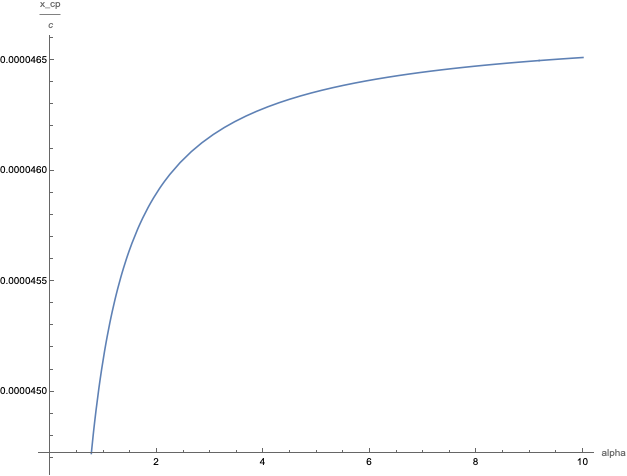
\includegraphics[width=0.75\textwidth]{images/s2.png}
		\end{center}
	\end{figure}

\end{homeworkProblem}

\begin{homeworkProblem}

	Given the pressure distribution \( p(x,y) = x^2+2y^2+50 \) acting on the body shown below, calculate the following:
	\begin{enumerate}
		\item The pressure force per unit depth on each face of the body.
		\item The magnitude and direction of the net force per unit depth on the body.
		\item The magnitude and direction of the net moment per unit depth on the body acting about the origin of the coordinate system.
		\item The location of the object's center of pressure with respect to the origin.
	\end{enumerate}

	\begin{figure}[ht]
		\begin{center}
			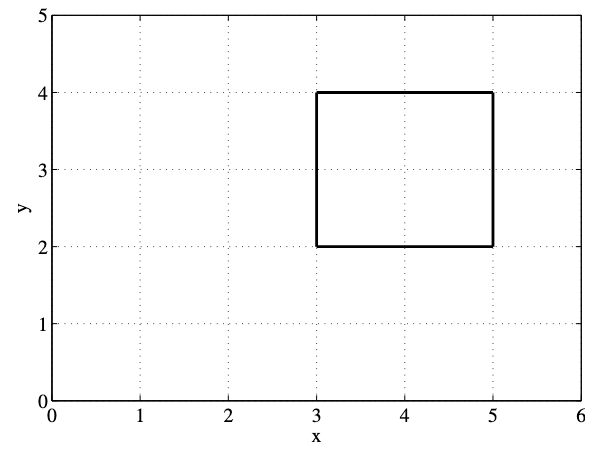
\includegraphics[width=0.65\textwidth]{images/p3.png}
		\end{center}
	\end{figure}

	\solution

	\part

	Face 1 coordinates: \( x=3, y=2:4 \).\\
	Face 2 coordinates: \( x=3:5, y=2 \).\\
	Face 3 coordinates: \( x=3:5, y=4 \).\\
	Face 4 coordinates: \( x=5, y=2:4 \).
	\begin{align*}
		p(x,y) & = x^2+2y^2+50                        \\
		F_{1}  & = \int^4_2 p(3,y) \dy = 155.333      \\
		F_{2}  & = \int^5_3 p(x,2) \dx = 148.667      \\
		F_{3}  & = \int^5_3 p(x,4) \dx = 196.667      \\
		F_{4}  & = \int^4_2 p(5,y) \dy = 187.333 \qed
	\end{align*}

	\part

	Net Force is given by the vector sum of the pressure force on each face.
	\begin{align*}
		\vec{F_{1}}+\vec{F_{2}}+\vec{F_{3}}+\vec{F_{4}}                                                                                                                          \\
		\vec{F} = \begin{bmatrix} F_{x} \\ F_{y} \end{bmatrix} = \begin{bmatrix} F_{1} & F_{4} \\ F_{2} & F_{3} \end{bmatrix} = \begin{bmatrix} 342.667 \\ 345.333 \end{bmatrix} \\
		\vec{F} = \sqrt{F_{x}^2+F_{y}^2} = 486.493, \ang{45.222} \qed
	\end{align*}

	\part

	Net Moment requires is given by reintegrating the pressure force on each face, now factoring in the distance from the origin of the coordinate system.
	\begin{align*}
		p(x,y)  & = x^2+2y^2+50                                                  \\
		M_{1}   & = \int^4_2 p(3,y)*3 \dy = 466                                  \\
		M_{2}   & = \int^5_3 p(x,2)*2 \dx = 297.333                              \\
		M_{3}   & = \int^5_3 p(x,4)*4 \dx = 786.667                              \\
		M_{4}   & = \int^4_2 p(5,y)*5 \dy = 936.667                              \\
		\vec{M} & = M_{1}-M_{2}+M_{3}-M_{4} = 18.667, \text{anti-clockwise} \qed
	\end{align*}

	\part

	\( COP \) can be calculated via \( \sum \frac{M_i}{F_i} \)
	\begin{align*}
		x_{cp} & = \frac{M_{1}+M_{4}}{F_{1}+F_{4}} = 4.0934 \\
		y_{cp} & = \frac{M_{2}+M_{3}}{F_{2}+F_{3}} = 3.1390 \\
		COP    & = (x_{cp}, y_{cp}) = (4.0934, 3.1390) \qed
	\end{align*}

\end{homeworkProblem}

\begin{homeworkProblem}

	Consider the steady flow of viscous incompressible fluid through a smooth, square pipe. The friction between the pipe wall and the fluid will result in a drop in pressure, \( \Delta p \), from one end of the pipe to the other that will depend on the length and width of the pipe, \( l \) and \( d \), the density and coefficient of viscosity of the fluid, \( \rho \) and \( \mu \), and the flow velocity, \( V \), i.e., \( \Delta p = f(l, d, \rho, \mu, V) \). Use the Buckingham Pi theorem to show that:
	\[
		\frac{\Delta p}{\rho V^2} = F(Re,\frac{l}{d}),
	\]
	where \( Re \) is the Reynolds number, \( Re = \frac{\rho V d}{\mu} \). If we extended the analysis to include pipe roughness (with a characteristic roughness height \( \epsilon \)), how would the above equation be modified?

	\solution

	\part

	Pressure drop \( \Delta p \) depends on the following:
	\begin{align*}
		\Delta p: & \left[ML^{-1}T^{-2}\right]   \\
		l:        & \left[ L \right]             \\
		d:        & \left[ L \right]             \\
		\rho:     & \left[ ML^{-3} \right]       \\
		\mu:      & \left[ ML^{-1}T^{-1} \right] \\
		V:        & \left[ LT^{-1} \right]
	\end{align*}
	We will repeat \( \rho, V, d \). Our dimensionless groups are as follows:
	\begin{align*}
		\pi_{1} = & \frac{\Delta p}{\rho V^{2}} \\
		\pi_{2} = & \frac{\rho V d}{\mu} = Re   \\
		\pi_{3} = & \frac{l}{d}
	\end{align*}
	We now have all of our dimensionless groups, and can relate \( \pi_{1} = F\left( \pi_{2}, \pi_{3} \right)\) \( \therefore \)
	\[
		\frac{\Delta p}{\rho V^2} = F(Re,\frac{l}{d}) \qed
	\]

	\part

	Now including the roughness, we need another dimensionless group:
	\[
		\pi_{4} = \frac{\epsilon}{d}
	\]
	This makes our new relationship \( \pi_{1} = F\left( \pi_{2}, \pi_{3}, \pi_{4} \right)\) \( \therefore \)
	\[
		\frac{\Delta p}{\rho V^2} = F(Re,\frac{l}{d}, \frac{\epsilon}{d}) \qed
	\]

\end{homeworkProblem}

\begin{homeworkProblem}

	Consider a long cylindrical wire that suddenly has a large electrical current passed through it, such that the wire explodes, depositing an energy per unit depth, \( E \), into the surrounding air. This causes a cylindrically expanding shock wave to propagate outwards from the initial position of the wire. If \( E \) is large, the initial propagation rate of this shock is independent of the pressure and temperature of the gas (this is known as the strong-shock limit); the only gas property that is important then is the density, \( \rho \).

	In fact, other thermodynamic properties of the quiescent air enter into the problem through the specific heats at constant volume and pressure, \( c_v \) and \( c_p \).
	\begin{enumerate}
		\item Using dimensional analysis, show that in the first case the shock velocity, \( V_s \), decays with time \( t \) as
		      \[
			      V_s = c \left( \frac{E}{\rho} \right)^{\frac{1}{4}} t^{-\frac{1}{2}},
		      \]
		      where \( c \) is a constant.
		\item In the second case, use the Buckingham Pi theorem to show that
		      \[
			      \frac{V_s^4t^2\rho}{E} = F(\gamma),
		      \]
		      where \( \gamma = \frac{c_{p}}{c_{v}} \).

	\end{enumerate}

	\solution

	\part

	Shock Velocity here depends on the following:
	\begin{align*}
		V_{s}: & \left[ LT^{-1} \right]  \\
		t:     & \left[ T \right]        \\
		E:     & \left[ MLT^{-2} \right] \\
		\rho:  & \left[ ML^{-3} \right]
	\end{align*}
	We want a relationship of the form:
	\[
		V_{s} = cE^{a}\rho^{b}t^{c}
	\], where \( a, b, c \) are constants.

	\[
		\left[M^{a} L^{a} T^{-2a}\right] \left[M^{b} L^{-3b}\right] \left[T^{c}\right] = \left[M^{a+b} L^{a - 3b} T^{-2a + c}\right] = \left[ LT^{-1} \right]
	\]

	As such, we can lay out the following:
	\[
		\left[
			\begin{array}[]{ccc|c}
				a  & b  & c & V_{s} \\
				\hline              \\
				1  & 1  & 0 & 0     \\
				1  & -3 & 0 & 1     \\
				-2 & 0  & 1 & -1
			\end{array}
			\right]
	\]
	We now have \( a = \frac{1}{4}, b = -\frac{1}{4}, c = -\frac{1}{2} \), giving us \( V_{s} = c E^{\frac{1}{4}} \rho^{-\frac{1}{4}} t^{-\frac{1}{2}} \) \( \therefore \)
	\[
		V_{s} = c \left( \frac{E}{\rho} \right)^{\frac{1}{4}} t^{-\frac{1}{2}} \qed
	\]

	\part

	For the Buckingham Pi theorem, we know Shock Velocity here depends on the following:
	\begin{align*}
		V_{s}: & \left[ LT^{-1} \right]           \\
		t:     & \left[ T \right]                 \\
		E:     & \left[ MLT^{-2} \right]          \\
		\rho:  & \left[ ML^{-3} \right]           \\
		c_{p}: & \left[ L^{2}T^{-2}K^{-1} \right] \\
		c_{v}: & \left[ L^{2}T^{-2}K^{-1} \right]
	\end{align*}
	As such, \( \gamma = \frac{c_{p}}{c_{v}} \) is dimensionless.

	We will repeat \( V_{s}, t, \rho \). Our dimensionless groups are as follows:
	\begin{align*}
		\pi_{1} = & \frac{V_{s}^{4}t^{2}\rho}{E} \\
		\pi_{2} = & \gamma
	\end{align*}
	Now, we simply have:
	\[
		\frac{V_s^4t^2\rho}{E} = F(\gamma) \qed
	\]

\end{homeworkProblem}

\end{document}
